\documentclass[logo,reportComp]{thesis}
\usepackage[cpp,linenum]{mypackage}

\title{计算机网络实验报告}
\subtitle{实验二:Echo实验}
\school{数据科学与计算机学院}
\author{陈鸿峥}
\classname{17大数据与人工智能}
\stunum{17341015}
\headercontext{计算机网络实验报告}

\begin{document}

\maketitle

\section{实验目的}
掌握套接字的基本使用方法

\section{实验说明}
\begin{itemize}
	\item 把源程序和可执行文件放在相应的上交源码目录中
	\item 截屏用按键(Ctrl+Alt+PrintScreen)截取当前窗口
\end{itemize}

\section{参考资料}
\begin{itemize}
	\item 套接字,\url{https://www.cnblogs.com/hgwang/p/6074038.html}
\end{itemize}

\section{实验环境}
本机为Ubuntu 18.04 (LTS) + gcc 7.3.0

\section{实验内容}
先尝试运行文件夹“TCP”中的程序:先运行Server程序(打开\verb'TCPServer.sln',然后执行)再运行Client程序(打开\verb'TCPClient.sln',然后执行)。
这两个程序的功能是客户端从服务器获取当前时间。

\textbf{由于本实验在Linux环境下进行,故没有按照上面步骤进行,但是Linux程序可正常编译运行。}

\subsection{TCP Echo程序}
\subsubsection{实验要求}
\textbf{服务器}把客户端发送来的任何消息都返回给客户端,返回的消息前面要加上服务器的当前时间。

\textbf{客户端}把返回的消息显示出来。
客户端每输入一条消息就建立TCP连接,并把消息发送给服务器,在收到服务器回应后关闭连接。

\subsubsection{运行结果}
\begin{itemize}
\item 客户端(两次运行)
\begin{figure}[H]
\centering
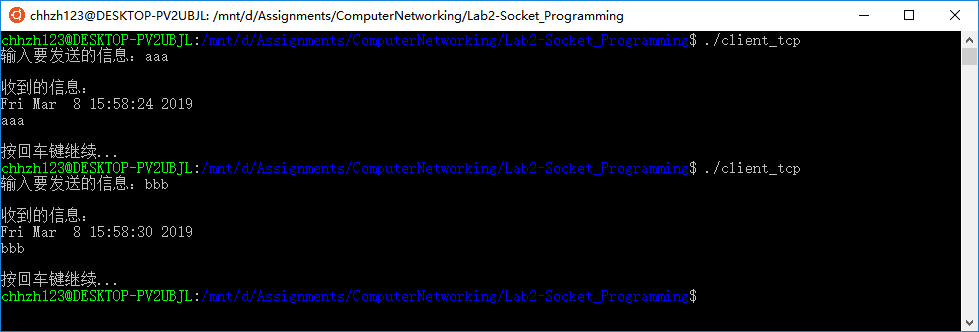
\includegraphics[width=0.8\linewidth]{fig/tcp-client.PNG}
\end{figure}
\item 服务器
\begin{figure}[H]
\centering
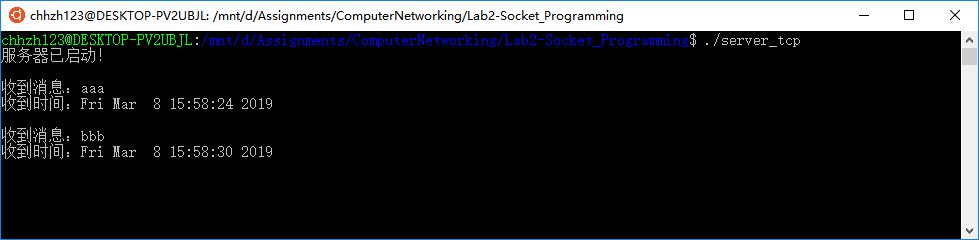
\includegraphics[width=0.8\linewidth]{fig/tcp-server.PNG}
\end{figure}
\item 只运行客户端程序而不运行服务器程序会出现什么错误,截屏并说明原因。
\begin{figure}[H]
\centering
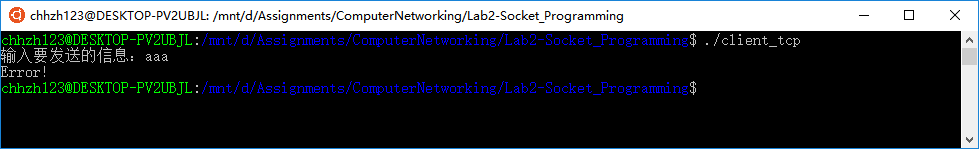
\includegraphics[width=0.8\linewidth]{fig/tcp-client-error.PNG}
\end{figure}
客户端的消息会发不出去,进而报错\verb'Error!'。
因为TCP是可靠的有连接的全双工传输协议,需要两侧同时建立连接才可以进行正常消息传递。
\item 服务器如何可以退出循环?\\
任意键入(由\verb'kbhit()'函数支持)或Ctrl+C
\end{itemize}

\subsubsection{服务器源代码}
注意\verb'kbhit()'函数未附在下面程序中。
\begin{lstlisting}
#include <sys/types.h>
#include <sys/socket.h>
#include <stdio.h>
#include <netinet/in.h>
#include <arpa/inet.h>
#include <unistd.h>
#include <stdlib.h>
#include <string.h>
#include <error.h>
#include <termios.h>
#include <unistd.h>
#include <fcntl.h>
#include <time.h>

#define BUF_LEN 2000

int kbhit(void);

void generateMsg(char* buffer){
    printf("`收到消息:'%s\n", buffer);

    time_t now; /* current time           */
    time(&now);
    char* pts = (char *)ctime(&now);
    printf("`收到时间:'%s\n", pts);

    strcat(pts,buffer);
    strcpy(buffer,pts);
    strcat(buffer,"\n");
}

int main(int argc, char *argv[])
{
    struct  sockaddr_in fsin;               /* the from address of a client   */
    int     msock, ssock;                   /* master & slave sockets         */
    char    *service = "50500";
    char    buf[BUF_LEN+1];                 /* buffer for one line of text    */
    struct  sockaddr_in sin;                /* an Internet endpoint address   */
    int     alen;                           /* from-address length            */
    char    *pts;                           /* pointer to time string         */

    // `创建套接字,参数:因特网协议簇(family),流套接字,TCP协议'
    // `返回:要监听套接字的描述符或INVALID\_SOCKET'
    msock = socket(PF_INET, SOCK_STREAM, IPPROTO_TCP);

    memset(&sin,'\0', sizeof(sin)); // `从'&sin`开始的长度为'sizeof(sin)`的内存清'0
    sin.sin_family = AF_INET; // `因特网地址簇'(INET-Internet)
    sin.sin_addr.s_addr = INADDR_ANY;                       // `监听所有(接口的)IP地址'
    sin.sin_port = htons((u_short)atoi(service));           // `监听的端口号'
    bind(msock, (struct sockaddr *)&sin, sizeof(sin));      // `绑定监听的IP地址和端口号'

    // `建立长度为5的连接请求队列,并把到来的连接请求加入队列等待处理'
    listen(msock, 5);

    printf("`服务器已启动!'\n\n");

    while (!kbhit()){ // `检测是否有按键,如果没有则进入循环体执行'
        alen = sizeof(struct sockaddr);                      // `取到地址结构的长度'
        // `如果在连接请求队列中有连接请求,则接受连接请求并建立连接,返回该连接的套接字'
        // `否则,本语句被阻塞直到队列非空。fsin包含客户端IP地址和端口号'
        ssock = accept(msock, (struct sockaddr *)&fsin, &alen);

        // `第二个参数指向缓冲区,第三个参数为缓冲区大小(字节数),第四个参数一般设置为0'
        // `返回值:(>0)接收到的字节数,(=0)对方已关闭,(<0)连接出错'
        int cc = recv(ssock, buf, BUF_LEN, 0);
        if (cc <= 0)
            printf("Error!\n"); // `出错或对方关闭(==0)。其后必须关闭套接字sock'
        else if (cc > 0) {
            buf[cc] = '\0';

            if (argc == 1){ // TCP Echo Enhancement
                generateMsg(buf);
            } else {
                generateEnhancedMsg(buf, (unsigned char *) &(fsin.sin_addr), fsin.sin_port);
            }

            cc = send(ssock, buf, strlen(buf), 0);
            if (cc <= 0)
                printf("Server send message error!\n");
        }

        close(ssock);
    }
    close(msock);
    return 0;
}
\end{lstlisting}

\subsubsection{客户端源代码}
\begin{lstlisting}
#include <sys/types.h>
#include <sys/socket.h>
#include <stdio.h>
#include <netinet/in.h>
#include <arpa/inet.h>
#include <unistd.h>
#include <stdlib.h>
#include <string.h>
#include <error.h>

#define BUF_LEN 2000

int main(int argc, char *argv[])
{
    char    *host = "127.0.0.1";       /* server IP to connect         */
    char    *service = "50500";        /* server port to connect       */
    struct  sockaddr_in sin;           /* an Internet endpoint address */
    char    buf[BUF_LEN+1];            /* buffer for one line of text  */
    int     sock;                      /* socket descriptor            */
    int     cc;                        /* recv character count         */

    // `创建套接字,参数:因特网协议簇(family),流套接字,TCP协议'
    // `返回:要监听套接字的描述符或INVALID\_SOCKET'
    sock = socket(PF_INET, SOCK_STREAM, IPPROTO_TCP);

    memset(&sin, 0, sizeof(sin)); // `从\&sin开始的长度为sizeof(sin)的内存清0'
    sin.sin_family = AF_INET;                         // `因特网地址簇'
    sin.sin_addr.s_addr = inet_addr(host);            // `设置服务器IP地址(32位)'
    sin.sin_port = htons((u_short)atoi(service));     // `设置服务器端口号'
    // `连接到服务器,第二个参数指向存放服务器地址的结构'
    // `第三个参数为该结构的大小,返回值为0时表示无错误发生'
    // `返回SOCKET\_ERROR表示出错,应用程序可通过WSAGetLastError()获取相应错误代码'
    int ret = connect(sock, (struct sockaddr *)&sin, sizeof(sin));

    printf("`输入要发送的信息:'");
    scanf("%s", buf);
    // `第二个参数指向发送缓冲区,第三个参数为要发送的字节数,第四个参数一般置0'
    // `返回值为实际发送的字节数,出错或对方关闭时返回SOCKET\_ERROR'
    cc = send(sock, buf, strlen(buf), 0);
    if (cc <= 0){
        printf("Error!\n");
        return 0;
    }

    printf("\n`收到的信息:'\n");
    if (cc <= 0)
        printf("Error!\n"); // `出错或对方关闭(==0)。其后必须关闭套接字sock'
    else if (cc > 0) {
        cc = recv(sock, buf, BUF_LEN, 0);
        buf[cc] = '\0';
        printf("%s\n", buf);
    }

    close(sock); // `关闭连接套接字'

    printf("`按回车键继续'...\n");
    getchar();
    return 0;
}
\end{lstlisting}

\subsection{TCP Echo增强程序}
\subsubsection{实验要求}
在上一实验的基础上,\textbf{服务器}在收到客户端的消息时显示服务器的当前时间、客户端的IP地址、客户端的端口号和客户端发来的信息,并把它们一并返回给客户端。

\textbf{客户端}在发送消息后把服务器发回给它的消息显示出来。(客户端程序与上一实验相同,不用修改)

要求服务器直接从\verb'accept()'的参数\verb'fsin'中得到客户端的IP地址和端口号。

注:服务器获取IP地址后要求直接使用\verb's_un_b'的四个分量得到IP地址,不能使用函数\verb'inet_ntoa()'转换IP地址。

\subsubsection{运行结果}
\begin{itemize}
\item 客户端(两次运行)
\begin{figure}[H]
\centering
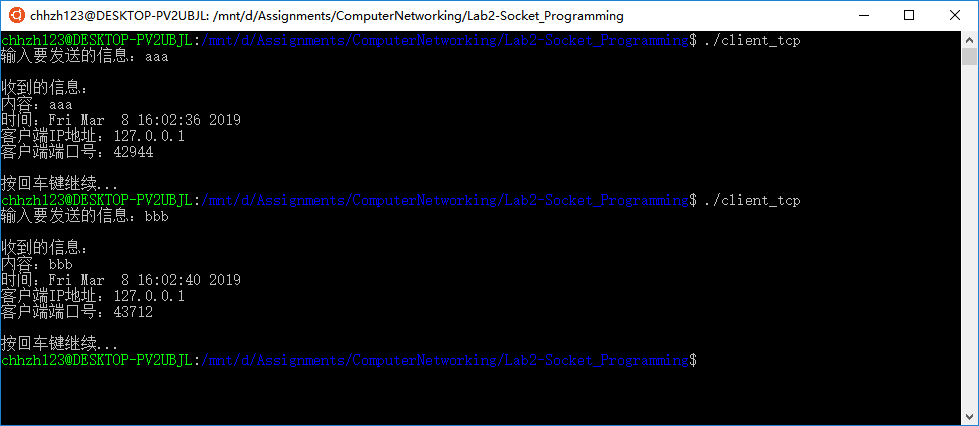
\includegraphics[width=0.8\linewidth]{fig/tcp-client-2.PNG}
\end{figure}
\item 服务器
\begin{figure}[H]
\centering
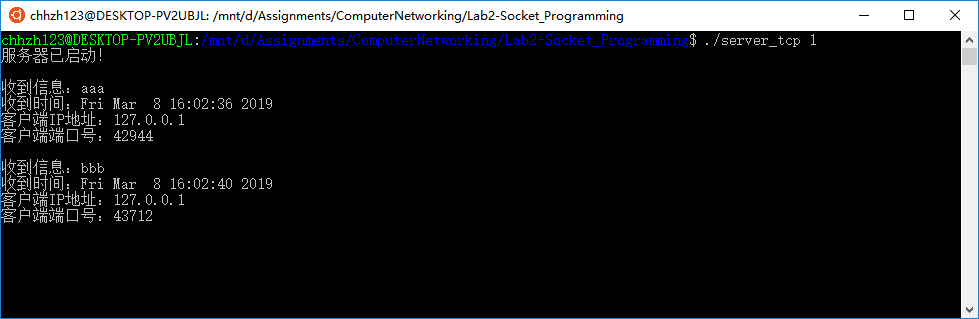
\includegraphics[width=0.8\linewidth]{fig/tcp-server-2.PNG}
\end{figure}
\end{itemize}

\subsubsection{服务器源代码}
只增加了一个消息生成函数,代码如下。
其他部分代码与原来的服务器相同,并且通过命令行读入参数,如果服务器程序命令行有参数读入,则执行增强版的程序。
\begin{lstlisting}
void generateEnhancedMsg(char* buffer, unsigned char *bytes, u_short port)
{
    char buf[BUF_LEN+1];
    printf("`收到信息:'%s\n", buffer);
    sprintf(buf, "`内容:'%s\n", buffer);

    time_t now; /* current time */
    time(&now);
    char* pts = (char *)ctime(&now);
    printf("`收到时间:'%s", pts);
    sprintf(buffer,"`时间:'%s", pts);
    strcat(buf, buffer);

    // inet_ntoa
    snprintf (buffer, sizeof (buf), "`客户端IP地址:'%d.%d.%d.%d\n",
              bytes[0], bytes[1], bytes[2], bytes[3]);
    printf("%s", buffer);
    strcat(buf,buffer);

    sprintf(buffer, "`客户端端口号:'%d\n", port);
    printf("%s", buffer);
    strcat(buf, buffer);

    printf("\n");
    strcpy(buffer,buf);
}
\end{lstlisting}


\subsection{UDP Echo增强程序}
\subsubsection{实验要求}
修改UDP例程,完成Echo功能,即当客户端发来消息时,服务器显示出服务器的当前时间、客户端的IP、客户端的端口号和客户发来的信息,并把它们一并发回给客户端,客户端然后把它们显示出来。

服务器可以直接从\verb'recvfrom()'的参数\verb'from'中得到客户端的IP地址和端口号,并且服务器用\verb'sendto()'发回给客户端消息时可以直接用该参数\verb'from'作为参数\verb'toAddr'。
可以使用\verb'inet_ntoa()'转换客户端IP地址。

客户端程序的\verb'recvfrom()'可以直接使用原来\verb'sendto'使用的\verb'sock'。
该\verb'sock'已经绑定了客户端的IP地址和端口号,客户端可以直接用来接收数据。


\subsubsection{运行结果}
\begin{itemize}
\item 客户端(两次运行)
\begin{figure}[H]
\centering
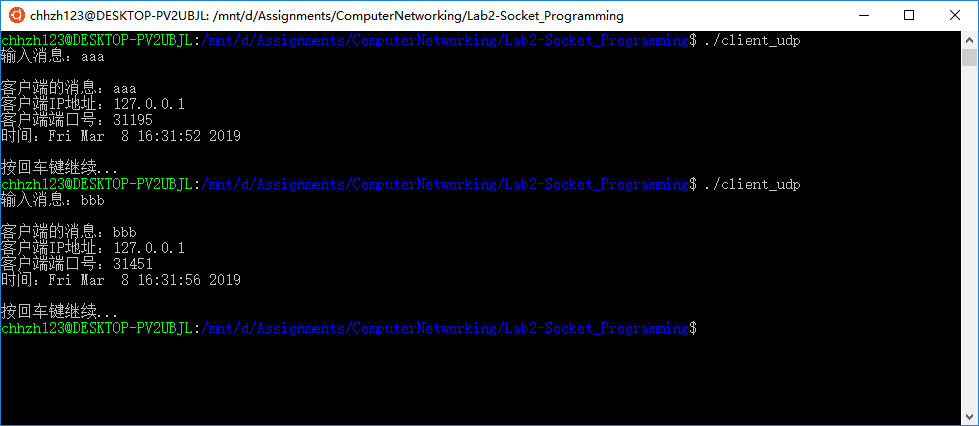
\includegraphics[width=0.8\linewidth]{fig/udp-client.PNG}
\end{figure}
\item 服务器
\begin{figure}[H]
\centering
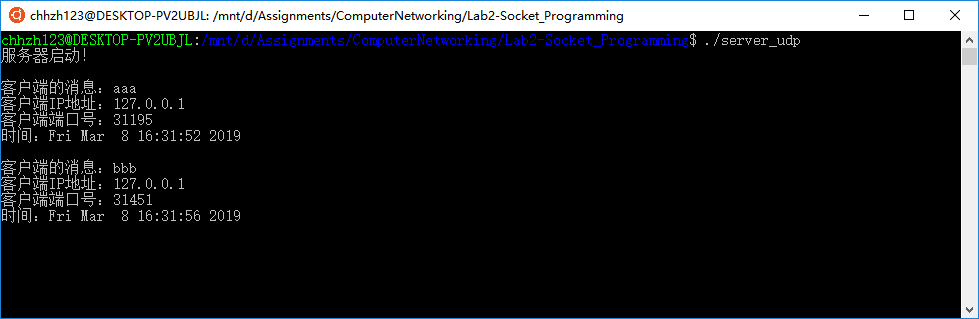
\includegraphics[width=0.8\linewidth]{fig/udp-server.PNG}
\end{figure}
\item 只运行客户端程序而不运行服务器程序会出现什么错误,截屏并说明原因。
\begin{figure}[H]
\centering
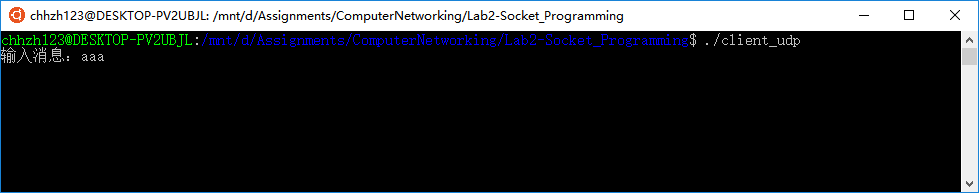
\includegraphics[width=0.8\linewidth]{fig/udp-client-error.PNG}
\end{figure}
客户端的消息可以正常发送,但发送完后会\textbf{一直等待}服务器返回信息。
因为UDP是不可靠的无连接的全双工传输协议(数据报),不需两侧同时建立连接就可以消息传递,但导致的结果就是丢包。
\end{itemize}

\subsubsection{服务器源代码}
\begin{lstlisting}
#include <sys/types.h>
#include <sys/socket.h>
#include <stdio.h>
#include <netinet/in.h>
#include <arpa/inet.h>
#include <unistd.h>
#include <stdlib.h>
#include <string.h>
#include <error.h>
#include <termios.h>
#include <unistd.h>
#include <fcntl.h>
#include <time.h>
 
#define BUFLEN   2000

int kbhit(void);

void generateEnhancedMsg(char* buffer, unsigned char *bytes, u_short port)
{
    char buf[BUFLEN+1];
    sprintf(buf, "`客户端的消息:'%s\n", buffer);
    printf("%s", buf);

    // inet_ntoa
    snprintf (buffer, sizeof (buf), "`客户端IP地址:'%d.%d.%d.%d\n",
              bytes[0], bytes[1], bytes[2], bytes[3]);
    printf("%s", buffer);
    strcat(buf, buffer);

    sprintf(buffer, "`客户端端口号:'%d\n", port);
    printf("%s", buffer);
    strcat(buf, buffer);

    time_t now; /* current time */
    time(&now);
    char* pts = (char *)ctime(&now);
    printf("`时间:'%s\n", pts);
    sprintf(buffer,"`时间:'%s", pts);
    strcat(buf, buffer);

    strcat(buf,"\n");
    strcpy(buffer, buf);
}

int main(int argc, char *argv[])
{
    char   *host = "127.0.0.1";        /* server IP Address to connect */
    char   *service = "50500";         /* server port to connect       */
    struct sockaddr_in sin;            /* an Internet endpoint address */
    struct sockaddr_in from;           /* sender address               */
    int    fromsize = sizeof(from);
    char   buf[BUFLEN+1];              /* buffer for one line of text  */
    int    sock;                       /* socket descriptor            */
    int    cc;                         /* recv character count         */

    // `创建UDP套接字, 参数:因特网协议簇(family),数据报套接字,UDP协议号'
    // `返回:要监听套接字的描述符或INVALID\_SOCKET'
    sock = socket(PF_INET, SOCK_DGRAM,IPPROTO_UDP); 
    printf("`服务器启动!'\n\n");

    memset(&sin, 0, sizeof(sin));
    sin.sin_family = AF_INET;
    sin.sin_addr.s_addr = INADDR_ANY;                     // `绑定(监听)所有的接口'
    sin.sin_port = htons((u_short)atoi(service));         // `绑定指定接口'
    // htons -- `主机序(host)转化为网络序(network), 为short类型'
    // `绑定本地端口号(和本地IP地址)'
    bind(sock, (struct sockaddr *)&sin, sizeof(sin));

    while(!kbhit()){ // `检测是否有按键'
        // `接收客户数据。返回结果:cc为接收的字符数,from中将包含客户IP地址和端口号'
        cc = recvfrom(sock, buf, BUFLEN, 0, (struct sockaddr *)&from, &fromsize);
        if (cc < 0){
            printf("recv() failed; %d\n", cc);
            break;
        } else {
            buf[cc] = '\0';
            generateEnhancedMsg(buf, (unsigned char *) &(from.sin_addr), from.sin_port);
            cc = sendto(sock, buf, strlen(buf), 0, (struct sockaddr *)&from, fromsize);
        }
    }
    close(sock);

    printf("`按回车键继续'...\n");
    getchar();
}
\end{lstlisting}

\subsubsection{客户端源代码}
\begin{lstlisting}
#include <sys/types.h>
#include <sys/socket.h>
#include <stdio.h>
#include <netinet/in.h>
#include <arpa/inet.h>
#include <unistd.h>
#include <stdlib.h>
#include <string.h>
#include <error.h>

#define BUFLEN 2000

int main(int argc, char *argv[])
{
    char   *host = "127.0.0.1";      /* server IP to connect         */
    char   *service = "50500";       /* server port to connect       */
    struct sockaddr_in toAddr;       /* an Internet endpoint address */
    int    tosize = sizeof(toAddr);
    char   buf[BUFLEN+1];            /* buffer for one line of text  */
    int    sock;                     /* socket descriptor            */
    int    cc;                       /* recv character count         */
    char   *pts;                     /* pointer to time string       */
    time_t now;                      /* current time                 */

    sock = socket(PF_INET, SOCK_DGRAM,IPPROTO_UDP);

    memset(&toAddr, 0, sizeof(toAddr));
    toAddr.sin_family = AF_INET;
    toAddr.sin_port = htons((u_short)atoi(service));
    // htons`:主机序(host)转化为网络序(network)', s--short
    toAddr.sin_addr.s_addr = inet_addr(host);
    // `如果host为域名,需要先用函数gethostbyname把域名转化为IP地址'

    printf("`输入消息:'");
    scanf("%s", buf);
    printf("\n");

    cc = sendto(sock, buf, BUFLEN, 0, (struct sockaddr *)&toAddr, sizeof(toAddr));
    if (cc <= 0) {
        printf("`发送失败,错误号:'%d\n", cc);
    } else {
        cc = recvfrom(sock, buf, BUFLEN, 0, (struct sockaddr *)&toAddr, &tosize);
        if (cc < 0){
            printf("recv() failed; %d\n", cc);
        } else {
            buf[cc] = '\0';
            printf("%s", buf);
        }
    }

    close(sock);

    printf("`按回车键继续'...\n");
    getchar();
}
\end{lstlisting}


\section{完成情况}
是否完成以下步骤?(\cmark 完成\quad\xmark 未做)\\
1. [\cmark]\qquad 2. [\cmark]\qquad 3.[\cmark]

\section{实验体会}
% 写出实验过程中遇到的问题,解决方法和自己的思考;并简述实验体会(如果有的话)。
本实验相对比较简单,有了实验一C字符串的铺垫,本实验做起来就比较得心应手,基本没有遇到什么问题。
本次代码编译在Linux环境下完成,会发现Linux环境下会方便很多,毕竟Linux内核就是用C写的。
而且Linux的命令行UTF-8编码也可以完美支持中文。

总的来说,通过本实验我明白TCP和UDP协议具体是怎么实施的,对C的字符串操作更加熟练了,而且会觉得计算机网络非常有趣,希望之后还可以继续做到这么有趣的实验。

\end{document}
% 【交实验报告】
% 每位同学单独完成本实验内容并填写实验报告。
%     交作业地点:http://172.18.187.9/netdisk/default.aspx?vm=17net 
% 编程实验 
% 截止日期:2019年3月16日23:00(周六)。
% 上传文件:学号_姓名_Echo实验报告.doc
% 学号_姓名_Echo实验源码.rar (源程序和可执行程序)